\chapter{Estado del Arte}
Tomando en consideración lo amplio, en el sentido de las disciplinas a abarcar, de este trabajo de tesis, el resumen del estado del arte para este se llevará a cabo en cuatro secciones distintas. 

Primero se expondrá la problemática que nace debido a la turbulencia en las simulaciones multiescala. Luego se revisará la historia y la creciente utilización de la técnica de Simulación de Grandes Vórtices (de aquí en adelante \emph{Large Eddy Simulations} o LES) en la solución numérica de los modelos meteorológicos. Tercero, se verán las complicaciones y los desafíos que conlleva el realizar simulaciones de alta resolución en terreno complejo y los consensos internacionales tomados al respecto. Finalmente se mostrará el estado actual de la utilización de los métodos de asimilación de datos para el uso operacional en el contexto de las simulaciones atmosféricas.
\section{Simulación Multiescala y Zona Gris}
Como ya se justificó en la introducción, la predicción atmósférica en zonas localizadas, en especial en aquellas con terreno irregular, es un tema de especial relevancia en las áreas del cambio climático, la contaminación ambiental y la industria energética. Actualmente las simulaciones climáticas regionales se realizan con una resolución de malla del orden de los kilómetros. Esto es, evidentemente, insuficiente para poder representar fehacientemente una topografía compleja, como puede ser la Cordillera de Los Andes, y por lo tanto, insuficiente también para resolver los fenómenos meteorológicos asociados a esta.

Una manera de solucionar esto puede ser el eso de un escalamiento estadístico para llevar las soluciones a una malla mas fina, sin embargo, este acercamiento no contempla ni la física fundamental ni las no-linealidades, que son la característica mas importante del comportamiento de la atmósfera. Su contraparte, el escalamiento dinámico, permite anidar mallas y resolver las leyes de conservación para resoluciones cada vez mas altas hasta lo que se desee resolver, teniendo como limitantes: el costo computacional, la precisión de las condiciones de borde y las parametrizaciones físicas que se incorporarán a las ecuaciones. Para este trabajo, es claro el beneficio que trae el utilizar el escalamiento dinámico como metodología para alcanzar simulaciones de alta resolución y por lo tanto ese es el acercamiento que se utilizará.

A modo de formar una explicación un poco mas formal y clara sobre lo que conlleva el realizar una simulación atmosférica multiescala, tomemos en consideración la Figura \ref{fig:escalas} para identificar las distintas escalas temporales y espaciales.

\begin{figure}[h!]
	\centering
	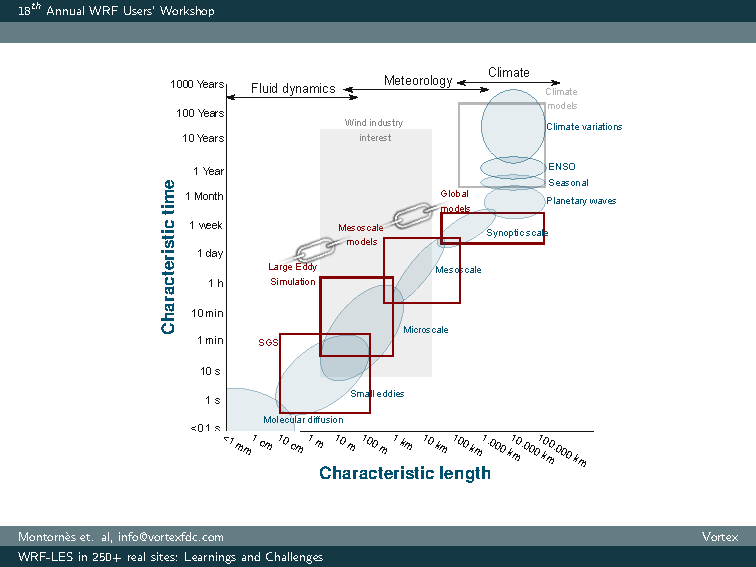
\includegraphics[width=0.85\linewidth,trim={2.6cm 1.4cm 1.5cm 0.8cm},clip]{Imagenes/01/terra}
	\caption{Separación de escalas para la dinámica atmosférica.}
	\label{fig:escalas}
\end{figure}

La figura en cuestión muestra tres aspectos claves de las simulaciones atmosféricas que se desean realizar: las áreas del conocimiento involucradas, los fenómenos que resuelve cada área y las escalas asociadas a cada uno de estas.

Nos referimos a simulación multiescala cuando, a través de algún proceso de escalamiento y simulación numérica se resuelven simultáneamente distintas escalas espaciales y se representan correctamente sus fenómenos asociados.
 
Nos referimos, por otra parte, a escalamiento dinámico, cuando se resuelven escalas mas pequeñas usando como base una escala mas grande, la cual es usada como condición inicial y de contorno en un subdominio de un dominio general. De esta forma es posible tener resultados numéricos para la microescala partiendo desde una escala, por ejemplo, global. 

En el contexto del trabajo a realizar, las escalas temporales pertenecientes a las simulaciones serán del orden de los días, por lo tanto, los fenómenos que se engloban dentro de estas son una combinación entre fenómenos de microescala, mesoescala y escala sinóptica. El buen comportamiento del resultado de una simulación estará directamente relacionado con lo bien representado que estén cada uno de estos fenómenos dentro del modelo.

De manera general, el escalamiento dinámico funciona bien y solo incorpora al modelo un error de interpolación debido al traspaso de una malla mas gruesa a otra mas fina. Sin embargo, la presencia de la turbulencia a lo largo de todo el espectro de escalas complica el escalamiento desde la mesoescala hasta la microescala.

Para entender la complejidad asociada a la presencia de la turbulencia debido al escalamiento dinámico, hay que entender primero la manera en la que actúan las distintas fuerzas que controlan el movimiento atmosférico. Si se considera, por ejemplo, la fuerza de Coriolis que es el motor principal de los ciclones y anticiclones en los hemisferios, esta fuerza es relevante en escalas sinópticas y globales y si se quisiera resolver ecuaciones a un nivel de mesoescala, podrían ser válidamente despreciadas. Por otra parte, si se considera ahora, la disipación viscosa generada por el roce entre los distintos elementos diferenciales de aire, esta podría ser válidamente despreciada también en todas las escalas debido a que la viscosidad del aire es muy baja, sin embargo si se desea analizar la parte viscosa de la capa límite atmosférica, este término es fundamental y no podría despreciarse\footnote{Un análisis mas detallado de las distintas fuerzas existentes dentro de las ecuaciones que modelan el comportamiento atmosférico se dará en el próximo capítulo}. 
 
Se concluye entonces que las distintas fuerzas que aparecen en las ecuaciones tienen un cierto rango de escalas propias donde contribuyen fuertemente al movimiento atmosférico. 

La turbulencia sin embargo\footnote{Probablemente le haga ruido al lector el hecho que hasta ahora no se ha presentado una definición formal de la turbulencia. Esta se presentará en el próximo capítulo.}, no funciona de la misma forma. Los vórtices de distintos tamaños que habitan en la atmósfera son igualmente importantes en términos de órdenes de magnitud para las ecuaciones que se resuelven.

Cuando se modelan las grandes escalas (sinóptica, mesoescala), generalmente la resolución de malla horizontal es demasiado grande como para captar los vórtices y por lo tanto en efecto de estos en las ecuaciones queda filtrado numéricamente. Operacionalmente, esta operación de filtrado se revierte con la utilización de un esquema adecuado para parametrizar la turbulencia. En los modelos meteorológicos actuales este efecto generalmente queda confinado en la llamada \emph{parametrización de capa límite}, ya que el principal rol que cumple la turbulencia en estas escalas es la de transmitir la información que se genera a nivel de superficie terrestre a la atmósfera libre.

Cuando se modelan las pequeñas escalas, idealmente la resolución de malla horizontal va a bastar para captar de manera adecuada cierto espectro de los vórtices generados por el efecto de la turbulencia y por lo tanto se puede omitir la parametrización de capa límite. Es importante notar que si bien ahora se resuelven los vórtices grandes que provocan la mezcla dentro de la capa límite, otra parte de los vórtices sigue sin ser resuelta y por lo tanto se deberá utilizar otro modelo turbulento para modelarla. Esta modelación será la encargada de representar la cascada de energía y la disipación de energía turbulenta.

\begin{figure}[h!]
	\centering
	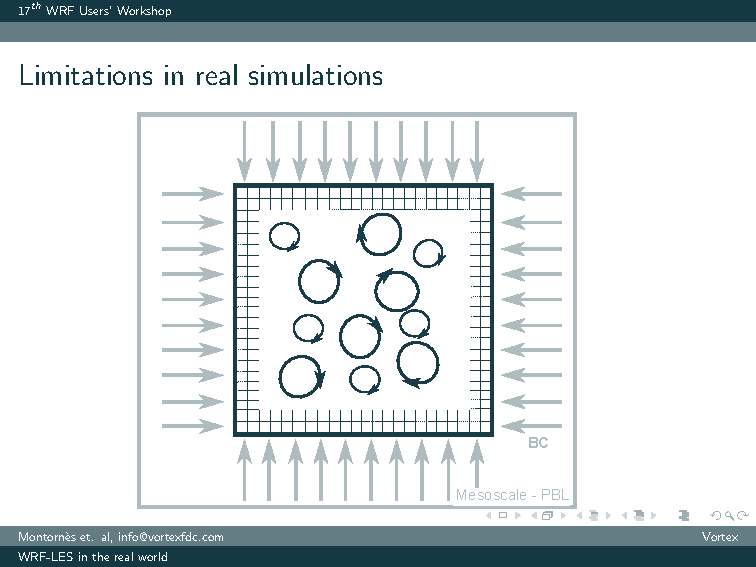
\includegraphics[width=0.5\linewidth,trim={2.67cm 1.05cm 3.1cm 1.98cm},clip]{Imagenes/01/grid}
	\caption{Idealización de los distintos tamaños de vórtices dentro de un dominio en la zona gris de la turbulencia. Los vórtices mas grandes pueden ser resueltos por la malla, mientras que los más pequeños son filtrados numéricamente y por lo tanto deben ser parametrizados para que su efecto se considere en las ecuaciones de movimiento.}
	\label{fig:01grid}
\end{figure}

Reflexionando un poco con respecto al rol que toma la turbulencia tanto en las escalas grandes como en las pequeñas, no es difícil llegar a la conclusión que a través del proceso de escalamiento dinámico se llegará eventualmente a una zona de traslape en donde algunos de los vórtices asociados a la capa límite son indistintamente resueltos y modelados al mismo tiempo. La Figura \ref{fig:01grid} representa este hecho. 

A esta zona de traslape se le denomina zona gris o \emph{Terra Incognita}.

Utilizando la terminología de Wyngaard (2004), sea $\Delta$ la escala (o tamaño) del filtro espacial asociado a la solución numérica (o malla) de las ecuaciones de movimiento y $l$ la escala característica de los vórtices en el rango inercial, el espectro de energía turbulenta $\phi(\lambda)$ se ve como se muestra en la Figura \ref{fig:terra}.

\begin{figure}[H]
	\centering
	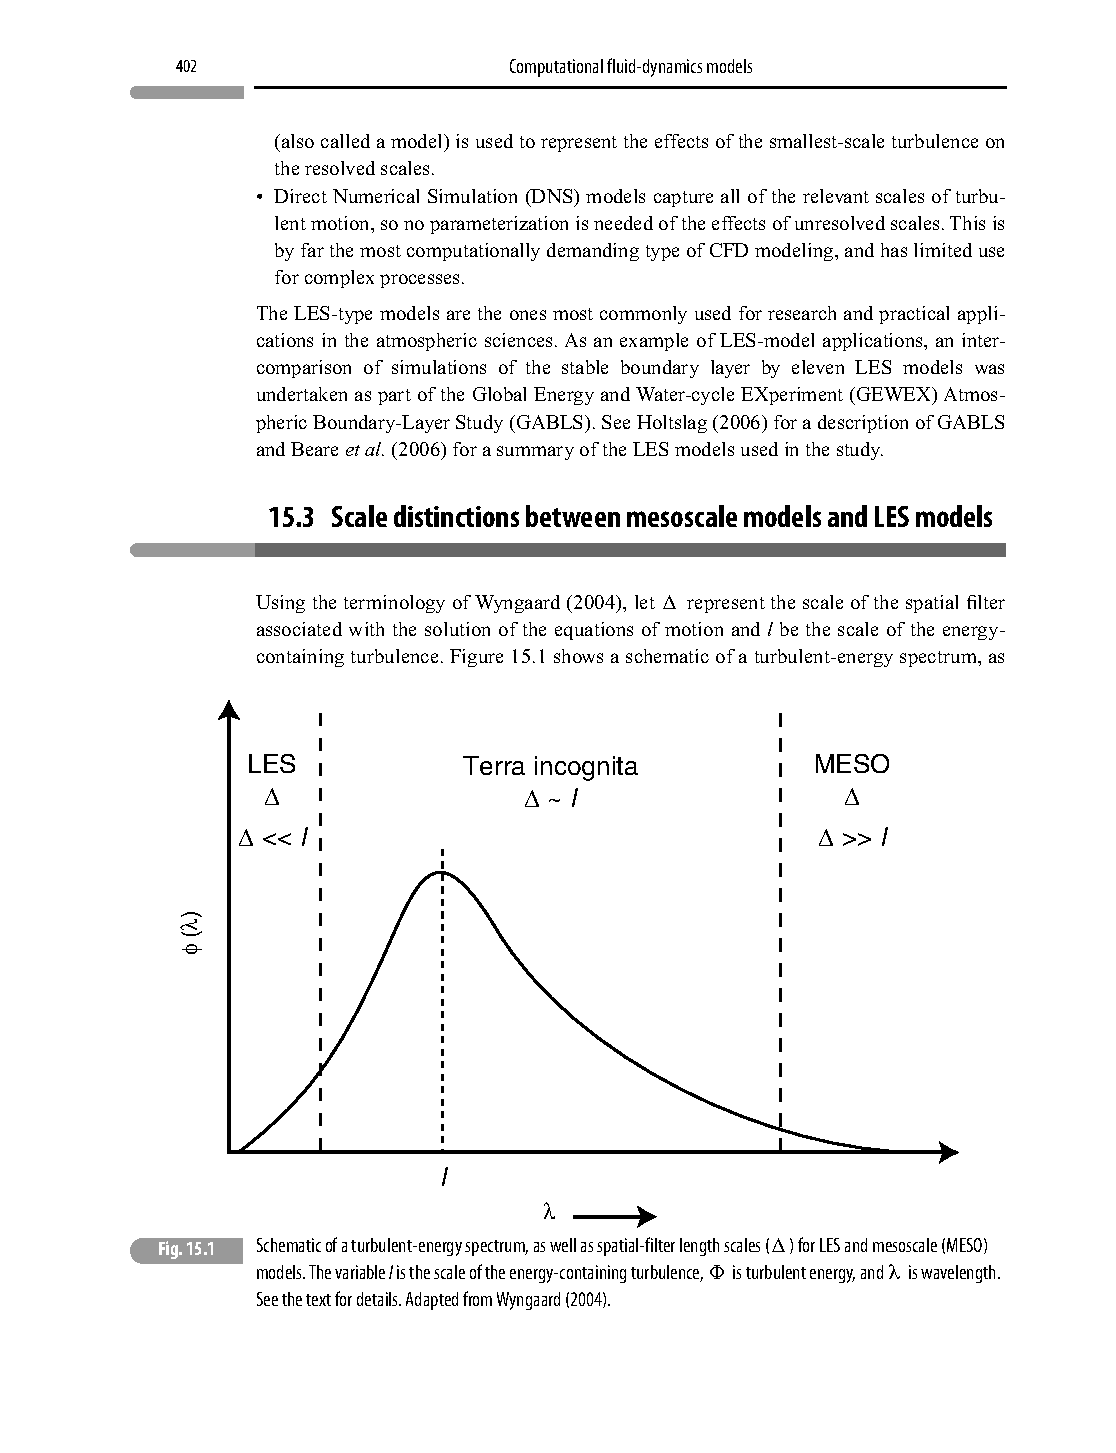
\includegraphics[width=0.8\linewidth,trim={2cm 3.0cm 1.5cm 11.5cm},clip]{Imagenes/terra}
	\caption{Espectro de energía turbulenta multiescala.}
	\label{fig:terra}
\end{figure}

Para valores de $\Delta\gg l$ asociados a la mesoescala, la producción de energía turbulenta queda por debajo del filtro y por lo tanto, tiene sentido que se modele a través de un esquema de submalla. Por otro lado, para valores de $\Delta\ll l$ los vórtices que contienen la energía pueden ser completamente modelado por las ecuaciones y entonces no debe usarse un SGS (microescala).

Queda entonces el rango en donde $\Delta\sim l$. Dentro de este intervalo se desconoce cual es el comportamiento de los modelos atmosféricos ya que existe una doble representación de tanto los vórtices que se resuelven como los que se modelan.

En la práctica, el acercamiento para compensar este problema es definir los dominios de modo que se evite usar el modelo en el rango de la \emph{Terra Incognita}.
\section{Turbulencia Atmosférica y LES}
\section{Simulaciones de Alta Resolución en Terreno Complejo}
\subsection{Importancia de la Estimación del Viento}
Para tener un acercamiento a la importancia de la correcta estimación del viento, consideremos la energía cinética del viento. Para un área arbitraria de magnitud $A$ en un tiempo $t$ se tiene:
\begin{equation} 
E = \frac{1}{2}mV^2 = \frac{1}{2}(AVt\rho)V^2 = \frac{1}{2}At\rho V^3
\end{equation}

Donde $\rho$ es la densidad del aire y $V$ es la rapidez del viento. $AVt$ es entonces el volumen de aire pasando por el área $A$ que se define como normal a la dirección de la velocidad del viento $V$. La potencia del viento (energía por unidad de tiempo) para el caso de una turbina eólica queda definida entonces como:
\begin{equation}
P = \frac{E}{t} = \frac{1}{2}A\rho V^3
\end{equation}

Donde $A$ pasa a ser ahora el área del rotor de la turbina. La potencia del viento, es entonces, proporcional al cubo de la velocidad del viento.

Se puede derivar la ecuación anterior para hallar una relación entre los errores relativos de las dos variables de interés. Derivando la ecuación anterior se obtiene:

\begin{equation}
dP = \frac{1}{2}A\rho\cdot d(V^3) = \frac{3}{2}A\rho V^2 dV
\end{equation}

Y dividiendo ahora por la potencia eólica:
\begin{equation}
\frac{dP}{P} = 3\frac{dV}{V}
\end{equation}

Lo que significa que un error relativo (o porcentual) en una estimación de la velocidad del viento, conlleva a un error el triple mas grande para la potencia que se podría generar.

\subsection{Problemáticas de la Simulación de Alta Resolución}

\section{Uso Operativo de Asimilación de Datos}

Como se verá mas adelante en detalle, el proceso de asimilación de datos corresponde a buscar la mejor  estimación del estado de la atmósfera a través de una combinación lineal entre un conjunto de observaciones y el resultado de un modelo. A esta estimación se le llama análisis.

Actualmente la asimilación de datos es ampliamente utilizada para corregir las desviaciones propias de las simulaciones de la dinámica atmósferica para los casos de las escalas globales y sinópticas, ya que para ese rango existen una gran cantidad de datos de acceso libre que se pueden utilizar.

Para este caso, como se busca mejorar la aproximación atmoserica de una zona a muy alta resolución, y en la capa límite, la colección de observaciones que uno pueda poseer siempre va a ser escasa y generalmente va a ser responsabilidad del equipo de modeladores implementar equipos de medición espeíficos para la zona. Es por esto la investigación acerca de la influencia de la asimilación de datos para estas escalas es limitada e incluso confidencial ya que su aplicación está relacionada con las empresas militares.



